\newpage
\section{Ergebnisse}
\label{sec:ergebnisse}
%Was waren die Ergebnisse der Untersuchungen?

In diesen Abschnitt werden die Ergebnisse zur Verdickungsmitteldosierung dargestellt. Nach Verifizierung des Problems und dessen Beschreibung erfolgen die Ergebnisse der Untersuchungsmethoden, sowie Entscheidungsverfahren für die Verfahrensplanung und schlussendlich die technische Umsetzung einer Dosiervariante mit einer Gefährdungsbeurteilung.

\subsection{Verifizierung und Analyse des Dosierproblems}
Im ersten Schritt wurde der Ist-Zustand der Dosierung erfasst, sowie die Gegebenheiten im Werk analysiert. Danach erfolgte das Zusammentragen der Anforderungen an eine halbautomatisch umgesetzte Dosierung.
 
\subsubsection{Ist-Zustand: Produktionsweise und aktuelles Dosierverfahren}
Das herzustellende Produkt für das eine halbautomatische Verdickerdosierung umgesetzt werden soll nennt sich \textit{AC 548}. Es ist eine Acrylat-Copolymer Dispersion und kann als Betonschutz, Fassadenfarben, wärmeaktivierbare Klebstoffe, Putze und Buntsteinputze verwendet werden. Produziert wird \textit{AC 548} im Batch-Betrieb à \SI{14}{\tonne} und die Planung erfolgt vorzugsweise in Kampagnen. \cite{ALBO.22.02.2022} \linebreak
Derzeit wird für dieses Produkt das Verdickungsmittel Rheobyk-H 3300 VF der \textsc{Byk-Chemie GmbH} eingesetzt, welches jedoch im Laufe des Jahres 2022 durch Einstellen der Produktion mit dem Verdickungsmittel TAFIGEL PUR 85 der \textsc{Münzing Chemie GmbH} substituiert werden soll. Die aktuelle Dosierung beläuft sich dabei auf die Nutzung eines \SI{0}{\liter}-Kunststofffasses als Dosierbehälter. Hierfür werden zunächst \SI{22}{\kilo \gram} des Verdickungsmittels in einem "`Transportfass"' im Chemikalienlager abgewogen und dann am entsprechenden Einstelltank bereit gestellt. Für den Start der Dosierung wird das "`Dosierfass"', welches mit einem Dosierloch an der Fassunterseite versehen ist, in das Fallschutzgitter des Mannlochs gehängt und der Inhalt des Transportfasses in das Dosierfass gekippt. Schematisch dargestellt ist diese Dosierung in Abbildung \ref{fig:aktuelle_dosierung}.

\begin{figure}[h!]
	\centering
	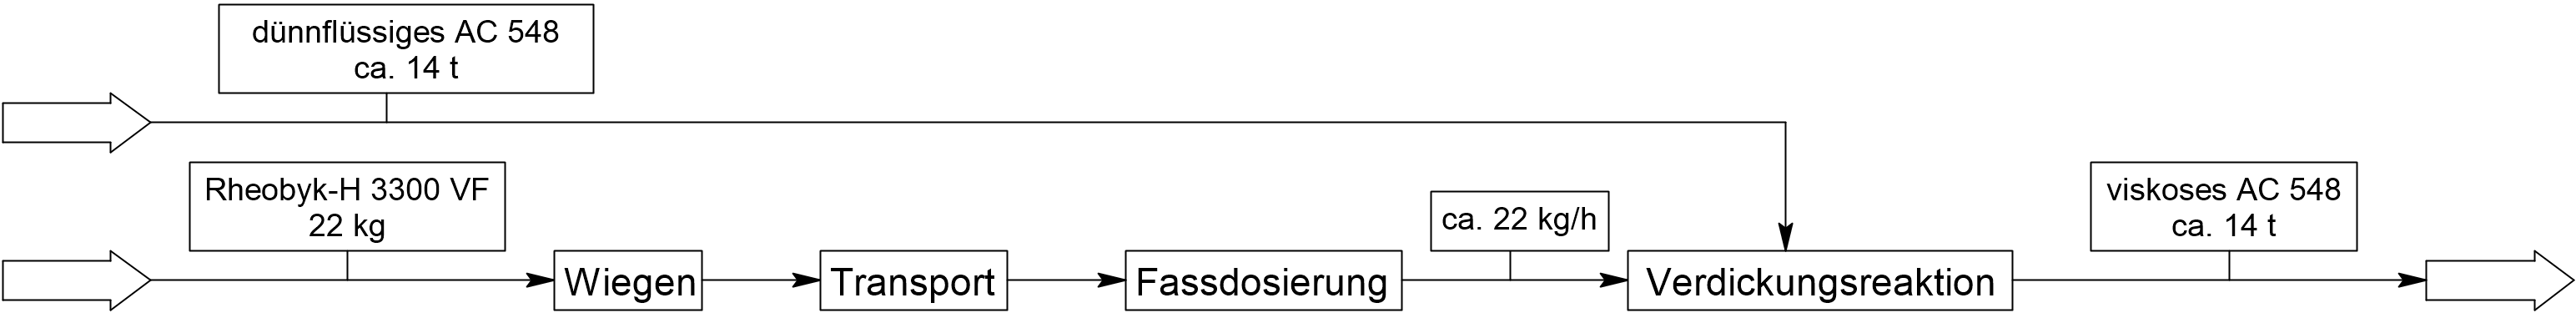
\includegraphics[width=\textwidth]{img/aktuelle_dosierung}
	\caption{Aktuelle Dosierung des Verdickungsmittels Rheobyk-H 3300 VF}
	\label{fig:aktuelle_dosierung}
\end{figure}
\FloatBarrier
%Ende

Vorteile dieses Dosierverfahrens sind die einfache und kostengünstige Umsetzung. Dem entgegen steht jedoch, dass neben dem "`Dosierloch"' und dem Fass selbst keine Einstellparameter vorhanden sind und der Dosierstrom weder messtechnisch erfasst noch im Prozessleitsystem (PLS) einsehbar ist. Zudem kann die Umsetzung für die Dosierung nur bedingt hygienisch erfolgen wie unter anderem in Abbildung \ref{fig:dosierfass} zu erkennen ist.

\begin{figure}[h!]
	\centering
	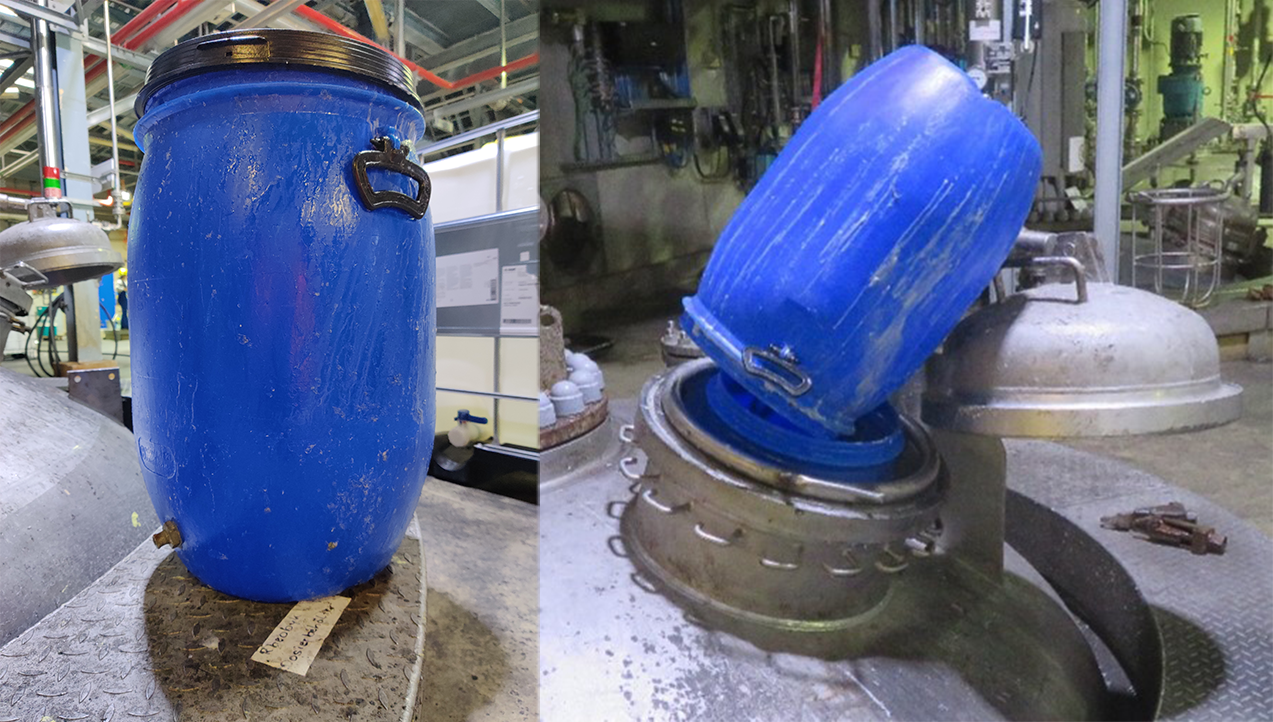
\includegraphics[width=0.5\textwidth]{img/dosierfass}
	\caption{Fotografien des Dosier- und des Transportfasses}
	\label{fig:dosierfass}
\end{figure}
\FloatBarrier
%Ende

\subsubsection{Soll-Zustand: Anforderung an die Dosierung}
Die Anforderungen an eine automatisierte Dosierung gliedern sich in mehrere Interessensgruppen auf. Beginnend mit der \textit{Technik}, sollen unter diesem Begriff jegliche Anforderungen der Prozess- und Sicherheitstechnik beschrieben sein. Beispielsweise fallen darunter die Dosierrate, die Dosiergenauigkeit und der zu beachtende Ex-Schutz. Die zweite Gruppierung beschreibt die Anforderungen der \textit{Produktion}, sprich die Interessen der auszuführenden Chemiefacharbeiter in der Anlage. Eine Forderung stellt dabei die einfache Bedienbarkeit dar. Zuletzt soll jedoch auch die \textit{Wartung} entsprechend leichtgängig und der Verschleiß des Dosiersystems gering sein. Die Forderungen aus den verschiedenen Perspektiven sind in Tabelle \ref{tab:anforderungen} zusammenfasst und wurden durch erfragen des Personals ermittelt und durch vorgegebenen Prozessparametern festgelegt.

% Table generated by Excel2LaTeX from sheet 'Daten'
\begin{table}[h!]
	\renewcommand*{\arraystretch}{1.2}
	\centering
	\caption{Anforderungen an die Verdickungsmittel-Dosierung}
	\label{tab:anforderungen}
	\resizebox{\textwidth}{!}{
		\begin{tabulary}{1.2\textwidth}{LL|L|L}
			\hline
			\multicolumn{2}{l|}{\textbf{Technik}} & \textbf{Produktion} & \textbf{Wartung}\\
			\hline
			Dosierrate: & 22 bis \SI{44}{\kilo \gram \per \hour}&einfache Bedienbarkeit&geringer Verschleiß\\
			Dosiergenauigkeit: & $\pm \, \SI{200}{\gram}$	& leichte Reinigung & leichte Wartung\\
			Ex-Schutz:	 & Zone 2 &Zeitersparnis&\\
			Risiko:  &minimal&&\\
			Verdickungsmittel: &TAFIGEL PUR 85&&\\
			Prozessleitsystem: &im PLS einsehbar&&\\
			Adaptierbarkeit:& für weitere Tanks adaptierbar &&\\
			Aufstellungsort: &siehe Abbildung \ref{fig:aufstellungsort}&&\\
			Einleitung: &siehe Abbildung \ref{fig:flansch}&&\\
			\hline
	\end{tabulary}}
\end{table}%
\FloatBarrier

Da weder die geforderte Dosiergenauigkeit erfasst, noch der Dosierstrom in der aktuellen Dosierung gemessen wird, ist eine signifikante Differenz zwischen Ist- und Soll-Anforderung an die Dosierung aus Perspektive der Technik erfüllt und das Dosierproblem somit als solches verifiziert. Die Perspektive der Produktion unterstützt diese Verifikation, da Anforderungen aufgrund der benötigten Vorbereitungszeit und der Sauberkeit der Dosierprozesses derzeit nicht erfüllt werden. Aus Sicht der Wartung besteht kein Handlungsbedarf.

\begin{figure}[h!]
	\begin{minipage}[b]{0.475\textwidth}
		\centering
		\includegraphics[height=4.25cm]{img/aufstellungsort}
		\caption{Aufstellungsort für Dosierung}
		\label{fig:aufstellungsort}
	\end{minipage}
	%\hspace*{0.05\textwidth}
	\begin{minipage}[b]{0.475\textwidth}
		\centering
		\includegraphics[height=4.25cm]{img/flansch}
		\caption{Flansch für eingehenden Dosierstrom}
		\label{fig:flansch}
	\end{minipage}
\end{figure}
\FloatBarrier

%geringer Verschleiß
%leichte Wartung
%einfach zu Bedienen
%leichte Reinigung --> Spülbarkeit
%Dosiergenauigkeit und DOsierstrom
%--> SAmmeln von Informationen im Werk
% Platz im Werk mit Geometrie
%
%Kampagne
%Mitarbeiterkosten sparen
%Zeitersparnis
%Einfachheit
%Ex-Schutz
%PLS
%Prozesssicherheit

\subsubsection{Ergebnisse der experimentellen Untersuchungen}
In der zu planenden Dosierung soll auf das Verdickungsmittel TAFIGEL PUR 85 der \mbox{\textsc{Münzing Chemie Gmbh}} zurückgegriffen werden. Laut Hersteller handelt es sich hierbei um einen assoziativen Polyurethan-Verdicker, welcher durch Gerüstbildung zwischen Verdickermolekülen, Bindemittel und Pigmentpartikeln die gewünschte Viskosität hervorruft und stabilisiert. Diese Beschreibung deckt sich mit der unter Abschnitt \ref{sec:grundlagen} formulierten Beschreibung der Assoziativverdicker. \cite{MunzingChemieGmbH.2014}
%--> Datenblätter
Die Ergebnisse der Viskositätsmessungen gliedern sich nach der Durchführung in Abschnitt \ref{sec:durchführung} in die Verifizierung der angegebenen Viskosität, der Untersuchung der Temperaturabhängigkeit, der Untersuchung der Verdünnungsabhängigkeit und in Pumpversuche.
Beginnend mit der Verifizierung der angegeben Viskosität sind in Abbildung \ref{dia:visko} die gemessenen Viskositäten des TAFIGEL PUR 85 und des Rheobyk-H 3300 VF dargestellt. 

%START DIAGRAMM

\begin{figure}[h]
	\begin{center}
		%\resizebox{\textwidth}{!}{
		\begin{tikzpicture}
			\begin{axis}[
				grid=both,
				grid style={line width=.1pt, draw=gray!10},
				major grid style={line width=.2pt,draw=gray!50},
				width= 0.95 \textwidth,
				height=0.5\textwidth,
				symbolic x coords={, Messreihe 1, Messreihe 2, Messreihe 3, Messreihe 4, Messreihe 5, \shortstack[c]{\SI{50}{\milli \liter} \\ Becherglas},},
				axis y line = left,
				axis x line = bottom,
				xtick=data,
				ytick={0,5,...,65},
				ymax = 65,
				ymin=0,
				ylabel=dynamische Viskosität in \si{\pascal \second},
				legend style={at={(0.475,1.05)},anchor=west},
				legend cell align={left}]
				%Tafigel
				\addplot[color=black,mark=*, only marks] coordinates {
					(Messreihe 1, 49.080)
					(Messreihe 2, 50.760)
					(Messreihe 3, 52.000)
					(Messreihe 4, 53.000)
					(Messreihe 5, 51.600)
					(\shortstack[c]{\SI{50}{\milli \liter} \\ Becherglas}, 50.87)
				};
				\addplot[color=black,dashed] coordinates {
				(Messreihe 1, 51.21)
				(\shortstack[c]{\SI{50}{\milli \liter} \\ Becherglas}, 51.21)
				};
				%Rheobyk
				\addplot[color=black,mark=o, only marks] coordinates {
					(Messreihe 1, 24.000)
					(Messreihe 2, 24.800)
					(Messreihe 3, 22.880)
					(Messreihe 4, 23.890)
					(Messreihe 5, 24.200)
					(\shortstack[c]{\SI{50}{\milli \liter} \\ Becherglas}, 23.32)
				};
				\addplot[color=black,dotted] coordinates {
					(Messreihe 1, 23.85)
					(\shortstack[c]{\SI{50}{\milli \liter} \\ Becherglas}, 23.85)
				};
			\legend{Viskosität - TAFIGEL PUR 85, Mittelwert (\SI{51}{\pascal \second}), Viskosität - Rheobyk-H 3300 VF, Mittelwert (\SI{24}{\pascal \second}) };
			\end{axis}
		\end{tikzpicture}
		%}
		\caption{Dynamische Viskositäten der Verdickungsmittel TAFIGEL PUR 85 und Rheobyk-H 3300 VF}
		\label{dia:visko}
	\end{center}
\end{figure} 

\FloatBarrier 
%ENDE

Die sich aus den Messwerten ergebenden Mittelwerte ergeben eine Viskosität für TAFIGEL PUR 85 mit \SI{51}{\pascal \second} und für Rheobyk-H 3300 VF \SI{24}{\pascal \second}. Zum Vergleich: Die Viskosität des TAFIGEL PUR 85 ist im Sicherheitsdatenblatt mit rund \SI{35}{\pascal \second}  angegeben. Auf Nachfrage beim Hersteller ist diese Schwankung produktionsbedingt und beeinträchtigt die Wirksamkeit des Verdickungsmittels nicht. \cite{MunzingChemieGmbH.2020} Ebenfalls zu erkennen ist, dass die Messwerte Abweichungen vom Mittelwert aufzeigen. Statistisch ergeben sich daraus relativen Standardabweichungen für die Messwerte des TAFIGEL PUR\,85 mit \SI{2,4}{\percent} und für das Rheobyk-H 3300 VF mit \SI{2,6}{\percent}. Die Messungen im \SI{50}{\milli \liter}, statt im \SI{600}{\milli \liter} Becherglas zeigten keine maßgeblichen Unterscheide.\linebreak
%--> nach DIN
%--> beide Verdickungsmittel
Eine weitere Untersuchung beschäftigte sich mit der Temperaturabhängigkeit des Verdickungsmittels. Dafür wurde zum einen der Verlauf der Dichte in Abhängigkeit von der Temperatur für das TAFIGEL PUR 85 bei der \textsc{Münzing Chemie GmbH} angefragt. Die erhaltenen Daten sind in Abbildung \ref{dia:dichte} zu sehen.

%START DIAGRAMM

\begin{figure}[h]
	\begin{center}
		%\resizebox{\textwidth}{!}{
			\begin{tikzpicture}
				\begin{axis}[
					grid=both,
					grid style={line width=.1pt, draw=gray!10},
					major grid style={line width=.2pt,draw=gray!50},
					width= 0.95 \textwidth,
					height=0.33\textwidth,
					%symbolic x coords={, Messreihe 1, Messreihe 2, Messreihe 3, Messreihe 4, Messreihe 5, \shortstack[c]{\SI{50}{\milli \liter} \\ Becherglas},},
					axis y line = left,
					axis x line = bottom,
					xtick={0,5,...,50},
					ytick={950,975,...,1050},
					xmax=50,
					ymax = 1050,
					ymin=950,
					xmin=0,
					ylabel=Dichte in \si{\kilo \gram \per \kmeter},
					xlabel = Temperatur in \si{\celsius},
					legend style={at={(1.0,0.95)},anchor=east},
					legend cell align={left},
					ylabel style={yshift=0.4cm},]
					%Tafigel
					\addplot[color=black,mark=*, only marks] coordinates {
						(10, 1034)
						(20, 1010)
						(30, 1008)
						(40, 1001)
					};				
					\legend{Dichte - TAFIGEL PUR 85};
				\end{axis}
			\end{tikzpicture}
			%}
		\caption{Dichte des TAFIGEL PUR 85 in Abhängigkeit von der Temperatur}
		\label{dia:dichte}
	\end{center}
\end{figure} 

\FloatBarrier 
%ENDE

Zu erkennen ist, dass sich die Dichte im Bereich zwischen 10 und \SI{40}{\celsius} mit steigender Temperatur verringert. Der Verlauf und der Umfang der Daten lässt nicht eindeutig auf einen linearen Zusammenhang zwischen Dichte und Temperatur schließen, jedoch ist erkennbar, dass ein signifikanter Unterschied in der Dichte für 10 und für \SI{40}{\celsius} besteht. Im Bereich zwischen 20 und \SI{30}{\celsius} bleibt die Dichte hingegen konstant. Aus den Daten wurde ermittelt, dass zwischen den Messungen eine relative Standardabweichung von \SI{1,4}{\percent} vorliegt.\linebreak
Neben dem Erfragen des Zusammenhangs zwischen Dichte und Temperatur ist auch die Abhängigkeit der Viskosität von der Temperatur untersucht worden. Der Grund hierfür liegt in der zuvor bestimmten Viskosität des Verdickungsmittels bei rund \SI{50}{\pascal \second}. Da im Regelfall bei der \textsc{Alberdingk Boley Leuna GmbH} keine so hohen Viskositäten gefördert werden, bot sich die Überlegung an die Viskosität durch Wärmezufuhr zu reduzieren. Das Ergebnis der dafür genutzten Versuchsreihe ist in Abbildung \ref{dia:temp} zu finden. Darin lässt sich erkennen, dass der Zusammenhang zwischen Viskosität und Dichte in diesem Temperaturbereich eine Linearität mit einem Bestimmtheitsmaß von \SI{99,6}{\percent} aufweist. Mit steigender Temperatur sinkt dabei die Viskosität. Der negative Anstieg lässt zudem darauf deuten, dass bei einer Temperaturerhöhung um \SI{5}{\kelvin} eine Verringerung der Viskosität um \SI{10}{\pascal \second} stattfindet.

%START DIAGRAMM

\begin{figure}[h]
	\begin{center}
		%\resizebox{\textwidth}{!}{
			\begin{tikzpicture}
				\begin{axis}[
					grid=both,
					grid style={line width=.1pt, draw=gray!10},
					major grid style={line width=.2pt,draw=gray!50},
					width= 0.95 \textwidth,
					height=0.4\textwidth,
					%symbolic x coords={, Messreihe 1, Messreihe 2, Messreihe 3, Messreihe 4, Messreihe 5, \shortstack[c]{\SI{50}{\milli \liter} \\ Becherglas},},
					axis y line = left,
					axis x line = bottom,
					xtick={0,5,...,50},
					ytick={0,5,...,65},
					xmax=50,
					ymax = 65,
					ymin=0,
					xmin=0,
					ylabel=dynamische Viskosität in \si{\pascal \second},
					xlabel = Temperatur in \si{\celsius},
					legend style={at={(1.,1.125)},anchor=east},
					legend cell align={left},
					%ylabel style={yshift=0.4cm},
					]
					%Tafigel
					\addplot[color=black,mark=*, only marks] coordinates {
						(21, 50.1)
						(25, 39.5)
						(30, 30.2)
						(35, 19.2)
						(39, 12.6)
					};
				
				\addplot [domain = 0:50, dashed] {-2.07*x+92.26};
							
					\legend{Viskosität - TAFIGEL PUR 85,$\eta(\vartheta) = -\SI{2,07}{\pascal \second \per \celsius}*\vartheta+\SI{92,26}{\pascal\second} \, | \, R^2 = \SI{99,6}{\percent}$};
				\end{axis}
			\end{tikzpicture}
			%}
		\caption{Dynamische Viskosität des TAFIGEL PUR 85 in Abhängigkeit von der Temperatur}
		\label{dia:temp}
	\end{center}
\end{figure} 
\FloatBarrier 
%ENDE
Zusätzlich wurde neben dem Aspekt der Erwärmung des Verdickungsmittels wurde auch der Effekt der Verdünnung auf die Viskosität untersucht. Es wird erwartet, dass mit sinkender Konzentration an Verdickungsmittel die Viskosität des Verdickungsmittels ebenfalls sinkt. In Abbildung \ref{dia:verdunnung} sind die Messergebnisse der Viskositäten beider Verdickungsmittel TAFIGEL PUR 85 und Rheobyk-H 3300 VF dargestellt. In separaten x-Achsen sind der Anteil an Verdickungsmittel und der Anteil an reiner Aktivsubstanz der Verdickungsmittels aufgetragen.

%START DIAGRAMM

\begin{figure}[h]
	\begin{center}
		%\resizebox{\textwidth}{!}{
			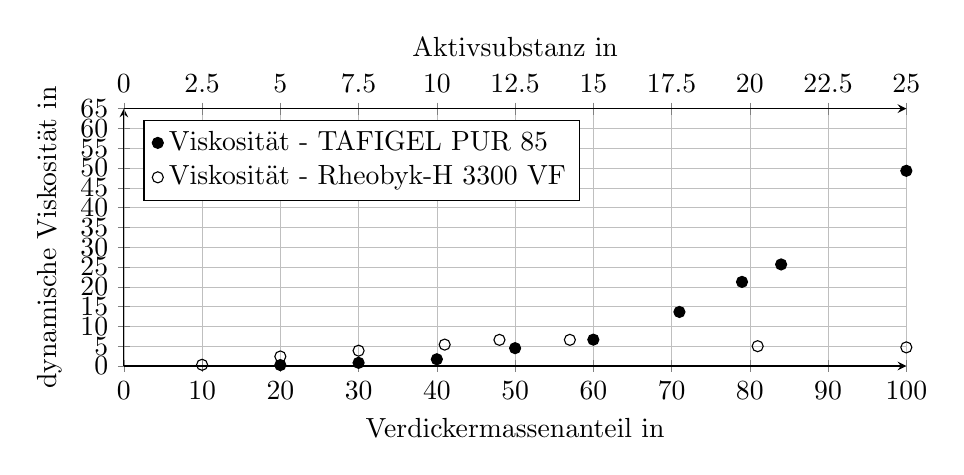
\begin{tikzpicture}
				\begin{axis}[
					grid=both,
					grid style={line width=.1pt, draw=gray!10},
					major grid style={line width=.2pt,draw=gray!50},
					width= 0.95 \textwidth,
					height=0.4\textwidth,
					%symbolic x coords={, Messreihe 1, Messreihe 2, Messreihe 3, Messreihe 4, Messreihe 5, \shortstack[c]{\SI{50}{\milli \liter} \\ Becherglas},},
					axis y line = left,
					axis x line = bottom,
					xtick={0,10,...,100},
					ytick={0,5,...,65},
					xmax=100,
					ymax = 65,
					ymin=0,
					xmin=0,
					ylabel=dynamische Viskosität in \si{\pascal \second},
					xlabel = Verdickermassenanteil in \si{\mpercent},
					legend style={at={(0.025,0.8)},anchor=west},
					legend cell align={left},
					%ylabel style={yshift=0.4cm},
					]
					%Tafigel
					\addplot[color=black,mark=*, only marks] coordinates {
						(20, .230)
						(30, .800)
						(40, 1.700)
						(50, 4.500)
						(60, 6.650)
						(71, 13.650)
						(79, 21.240)
						(84, 25.650)
						(100, 49.300)
					};
				%Rheobyk
				\addplot[color=black,mark=o, only marks] coordinates {
					(10, 0.300)
					(20, 2.400)
					(30, 3.870)
					(41, 5.400)
					(48, 6.600)
					(57, 6.600)
					(81, 5.000)
					(100, 4.700)
	
				};
					\legend{Viskosität - TAFIGEL PUR 85, Viskosität - Rheobyk-H 3300 VF};
				\end{axis}
			\begin{axis}[
				width= 0.95 \textwidth,
				height=0.4\textwidth,
				%symbolic x coords={, Messreihe 1, Messreihe 2, Messreihe 3, Messreihe 4, Messreihe 5, \shortstack[c]{\SI{50}{\milli \liter} \\ Becherglas},},
				hide y axis,
				axis x line = top,
				xtick={0,2.5,...,25},
				xmax=25,
				xmin=0,
				xlabel = Aktivsubstanz in \si{\mpercent},
				legend style={at={(1.,1.125)},anchor=east},
				legend cell align={left},
				]
				%Tafigel
				\addplot[draw=none, forget plot] coordinates {
					(5, .230)
					(7.5, .800)
					(10, 1.700)
					(12.5, 4.500)
					(15, 6.650)
					(17.7, 13.650)
					(19.9, 21.240)
					(20.9, 25.650)
					(25, 49.300)
				};
			\end{axis}
			\end{tikzpicture}
			%}
		\caption{Dynamische Viskositäten der Verdickungsmittel  TAFIGEL PUR 85 und Rheobyk-H 3300 VF in Abhängigkeit vom Massenanteil des Verdickungsmittels bzw. dem Anteil an Aktivsubstanz}
		\label{dia:verdunnung}
	\end{center}
\end{figure} 
\FloatBarrier 
%ENDE
Durch dieses Diagramm zeigt sich, dass sich beide Verdickungsmittel in ihrem Verdünnungsverhalten deutlich unterscheiden. Während das Rheobyk-H 3300 VF ab \SI{40}{\mpercent} eine vergleichsweise stabile Viskosität in Abhängigkeit von der Verdünnung aufzeigt, lässt sich für das TAFIGEL PUR 85 eine starke Abhängigkeit zwischen Viskosität und Verdickermassenanteil festzustellen. Auffallend ist zudem, dass die Viskosität des Rheobyk-H 3300 VF im Bereich zwischen 50 und \SI{60}{\mpercent} höher ist als mit einem Verdickeranteil von \SI{100}{\mpercent}.
%
%\subsubsection{Verdünnungsverhalten}
%%--> Eigenregie
%
%\subsubsection{Erwärmungsverhalten}
%%--> beim Hersteller angefragt
%
Im Laufe der Überlegungen zur Umsetzung der Dosierung wurde die Möglichkeit der Dosierung mit einer Pumpe in Betracht gezogen. Durch die hohen Viskosität und den Anforderungen an Sauberkeit und Wartung, sollte zunächst die Pumpbarkeit des TAFIGEL PUR 85 mit einer Schlauchpumpe überprüft werden. Die Ergebnisse der Massenströme bei verschiedenen Drehzahlen ist im Diagramm unter Abbildung \ref{dia:pumpe} gezeigt.



\subsubsection*{Pumpversuche}

erster Volumenstrom erst nach einer Stunde zu erkennen 


\todo[inline]{Entscheidungsprobleme werden aufgrund des Umfangs und der schweren Nachvollziehbarkeit nicht dargestellt}

\subsection{Entscheidungsprobleme}
\label{subsec:entscheidungsprobleme}
\subsubsection{Entscheidung für ein Verfahren}
%Verdünnen
%spülen
%erwrämen
%nichts 
%Rühren
%kombinationen
%aktuelles Verfahren

\subsubsection{Entscheidung für Gebindetyp}
%Preis nachfrage
%\subsubsection{Angebotsanfrage}
%\subsubsection{Entscheidungsverfahren}

\subsubsection{Entscheidung für Pumpendosierung oder Dosierbehälter}

\subsubsection{Auswahl des Pumpentyps}
%\subsubsection{Literaturarbeit}
%Bücher gelesen für Auswahlhilfe
%\subsubsection{Fachgespräche und Angebotsanfrage}
%\subsubsection{Entscheidungsverfahren}

%\subsection{Auswahl des Pumpentyps, sowie des Leitungsdurchmessers}
%Gespräche geführt und Leitung hat sich nach möglichen Drücken in der Anlage und Pumpentyp, sowie Berechnungen gerichtet gerichtet

\subsubsection{Auswahl des Messverfahrens}

\subsection{Technische Planung für Verdickungsmitteldosierung}
\subsubsection{Verfahrensfließbild der Verdickerdosierung}
\subsubsection{R\&I- Fließbild der Verdickerdosierung}
\subsubsection{Rohrleitungsplanung der Verdickerdosierung}
%vertretbarer Druckverlust
%Rohrdurchmesser und Nenndruck
%--> Rohrleitungsklassifizierung

\subsubsection{EMSR-Plan der Messtechnik für die Dosierung}

\subsection{Gefährdungsbeurteilung der geplanten Verdickungsmitteldosierung}


